\section{R-CNN}

R-CNN, also known as regional-based convolutional neural networks, is an object detection algorithm. The algorithm was developed by a group of researchers at UC Berkeley in 2015. Since its development, the R-CNN model has revolutionized the field of computer vision. The model was designed to detect up to 80 different types of objects in images and provide large-scale object recognition capabilities. Additionally, before the existence of RCNN, most algorithms in object recognition task used support vector machine (SVM) with blockwise orientation histograms like Histogram of Oriented Gradients (HOG) or Scale-Invariant Feature Transform (SIFT). SVM dominated the space until 2012. In 2012, a CNN algorithm showed an astounding image classification accuracy on ImageNet Large Scale Visual Recognition Challenge (ILSVRC). Since then, more studies have been created into developing and improving algorithms utilizing CNN. The R-CNN model is our first attempt to build an object detection model that extracts features using a pre-trained CNN.

In a board picture, R-CNN model is composed of three modules (Figure \ref{fig:rcnn_archiet}). The first module's purpose is to generate regions of interest (ROI) i.e., regions that possibly contain an object. The second module utilizes a CNN to extract out feature vector from each proposed region. The third module then performs classification for each region using a pre-trained SVM algorithm on the feature vectors provided by the second module. As we can see R-CNN algorithm tries to find the location of each object, extract the object features, and classify these features. Next, we will dive deeper into each module of R-CNN.

\begin{figure}[!ht]
    \centering
    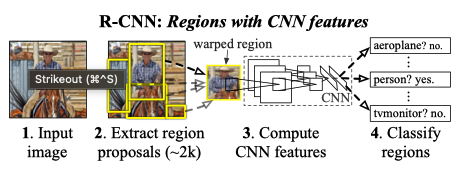
\includegraphics[width=4.5in]{figures/rcnn_archiet.png}
    \caption{R-CNN Overall Architecture \cite{Girshick_R_CNN_2013}} \label{fig:rcnn_archiet}
\end{figure}

\subsection{The First Module: Region Proposal}
In the first module, the algorithm used in this step must be able to propose some region of interest (ROI). A region of interest is a smaller part of the original image that could contain an object.

Given this problem, one might consider the bruce-force method by examining every small rectangle area of the original image as a potential region of interest in a systematic way. This method is the main concept behind the sliding-window technique, a type of exhaustive search algorithm used in the region proposal task. The sliding window technique involves running a window of a predefined size across the image, such that each subsection of the image is considered as a potential region proposal. Like the CNN kernel, the windows' size, stride, and padding are all customizable and can be adjusted to suit different types of images. In addition, multiple scales can also be incorporated into the sliding window technique, which allows for more robust performance in scenarios where objects may appear at different sizes within the same image. Since the sliding window technique examines every location within the image by considering every pixel as part of some ROI, it will not miss any potential object location. However, considering every location in the image as a ROI is unnecessary due to objects most likely not appearing everywhere in the image. Furthermore, classifying every sub-image at different sizes will require tremendous computational power. Therefore, even though it allows our model to detect all possible locations, the sliding window technique should not be used in autonomous cars' vision because it is computationally expensive.

{\color{red} consider describe segmentation statregy: segmentation able to generate multiple foreground and background segmentation and is trained to scoring if a forground segment is an object}

In recent years, many study have show interest in improve the efficient of region proposal algorithm. One notable algorithm that given the same strength as the sliding window technique is selective search. Selective search was designed to combines the strength of both exhaustive search and segmentation \cite{uijlings_selective_search_2013}. The strength that selective search inherits from sliding windows is the ability to find all the possible locations that can be a potential region of interest. Additionally, selective search ustilize the underlying image structure to cluster pixels into different regions, taken from the strength of segmentation technique. Selective search also aim to complete three goals. These three goals are capture all scale, diversification, and fast to compute. Capture all scale is the idea that the algorithm must be able to detect object at different size in the image. Next, diversification requirement refer to method of grouping region. The algorithm must be able to combine region contain part of an object into one region. Additionally, for instance like a person inside a car or person in front of a car, the algorithm must be able to seperate the region for the car and the region for the person under diversification requirement. Lastly, fast to compute require the algorithm to not demain heavy computational power.

As for selective search overall behavior. It can be thought as two steps. The first step is perform bottom-up segmentation -- descibed in Efficient Graph-Based Image Segmentation by Felzenszwalb and Huttenlocher \cite{felzenszwalb_huttenlocher_2004} -- to generate initial sub-segmentation. The second step is combine similar sub-segmentation recursive using a similarity score between subsegment. The similarity score is a combination of four similarity grouping criteria. These four criteria are color similarity, texture similarity, size similarity, and fill similarity \cite{uijlings_selective_search_2013}. The reason that color and texture similarity between regions is needed is due to same object mostlily will have the same texture or shade of color. In the original paper, the color and texture similarity criteria score can be descibed by an equation only based on fixed number of values taken from histogram of each color channel. Thus, these two similarity score require minimal to no computational power to compute. Similarly, two region that have majority of the area overlap on each other are most likely described the same object. Therefore, the use of fill similarity score allow the algorithm to merge regions that are mostly overlap and keep regions that are not overlaping seperate from each other. The fill similarity score can be caculated using the following equation: 
%
\begin{equation*}
    S_{fill}(r_i, r_j) = 1-\frac{size(BB_{ij})-size(r_i)-size(r_j)}{size(image)}
\end{equation*}
%
where $r_i, r_j$ are two considering ROI, and $BB_{ij}$ is the bounding box around $i$ and $j$. Lastly, the similarity in size between two regions take into consideration to make sure ensures that the algorithm identify all locations for different object at different scale. The size similarity score can be caculated using the following equation: 
%
\begin{equation*}
    S_{size}(r_i, r_j) = 1-\frac{size(r_i)+size(r_j)}{size(image)}
\end{equation*}
%
where $r_i, r_j$ are two considering ROI. As we can see, the similarity score computation is fast and take into accout the diversify of the image data set. With this two steps, selective search can quickly classify foreground and background, then downsampling number of potential ROI existed in forground segmentation. Therefore, by utilize selective search allow the model to reduce number of falsify ROI compare to sliding window and require lower computational power.

In the original paper of R-CNN, in the first module -- region proposal -- utilize selective search algorithm \cite{Girshick_R_CNN_2013}. However, as mention before, the R-CNN model can be thought of as three seperate modules, thus one can experiment R-CNN with different region proposal technique.

\subsection{The Second Module: Feature Extraction With CNN}
On completion of the first module of R-CNN, which generates all regions of interest within an image, these ROIs are passed to the AlexNet architect for feature extraction \cite{Girshick_R_CNN_2013}. AlexNet, a CNN architect, was proposed by Alex Krizhevsky at the University of Toronto in 2012 with the guidance of Ilya Sutskever and Geoffrey E. Hinton \cite{AlexNet_2017}. AlexNet was trained using ImageNet, which at the time was the most extensive picture data collection. As AlexNet required its input to have a fixed resolution with the same width and height, the photos in ImageNet were resized to $256 \times 256$ pixels. Prior to publication, AlexNet competes in ILSVRC-2010 and obtained top-one error rates of 37.5\%. In other words, 37.5\% of the time, the model assigns the highest score to the correct label.  In the same competition, AlexNet also achieves top-5 error rates of 17.0\%, i.e., the correct label in the top 5 predicts 17\% of the time.

% \subsubsection{AlexNet}
AlexNet is regarded as one of CNN's most significant innovations. AlexNet, with 60 million parameters and 650,000 neurons as of 2012, is one of the largest neural networks ever suggested. The architecture of AlexNet consists of eight learned layers. Five convolutional layers are followed by three layers that are fully connected. Due to hardware limitations at the time, it was not possible to fit a massive network like AlexNet on a single GPU. For this reason, the model's architecture is distributed across two separate GPUs, and training must pass via both GPUs. Due to this limitation, for each layer in the network, the model has half of the neurons for that layer on each GPU and only requires particular layers to perform GPU communication. For example, in the overall architecture of AlexNet presented in Figure \ref{fig:alex_net_architecture}, we note that neurons of the first layer only connect to neurons of the second layer on the same GPU. On the contrary, we notice that all neurons of the second layer are fully connected with neurons in the third layer. The notion of spreading neurons across multiple GPUs is known as the parallelization scheme. The parallelization scheme is a topic that remains outside the scope of this paper, and GPU memory size is no longer a significant problem due to the current advancement of technology. Therefore, understanding the parallelization scheme is likely to be optional for the analysis of a CNN model.

\begin{figure}[!ht]
    \centering
    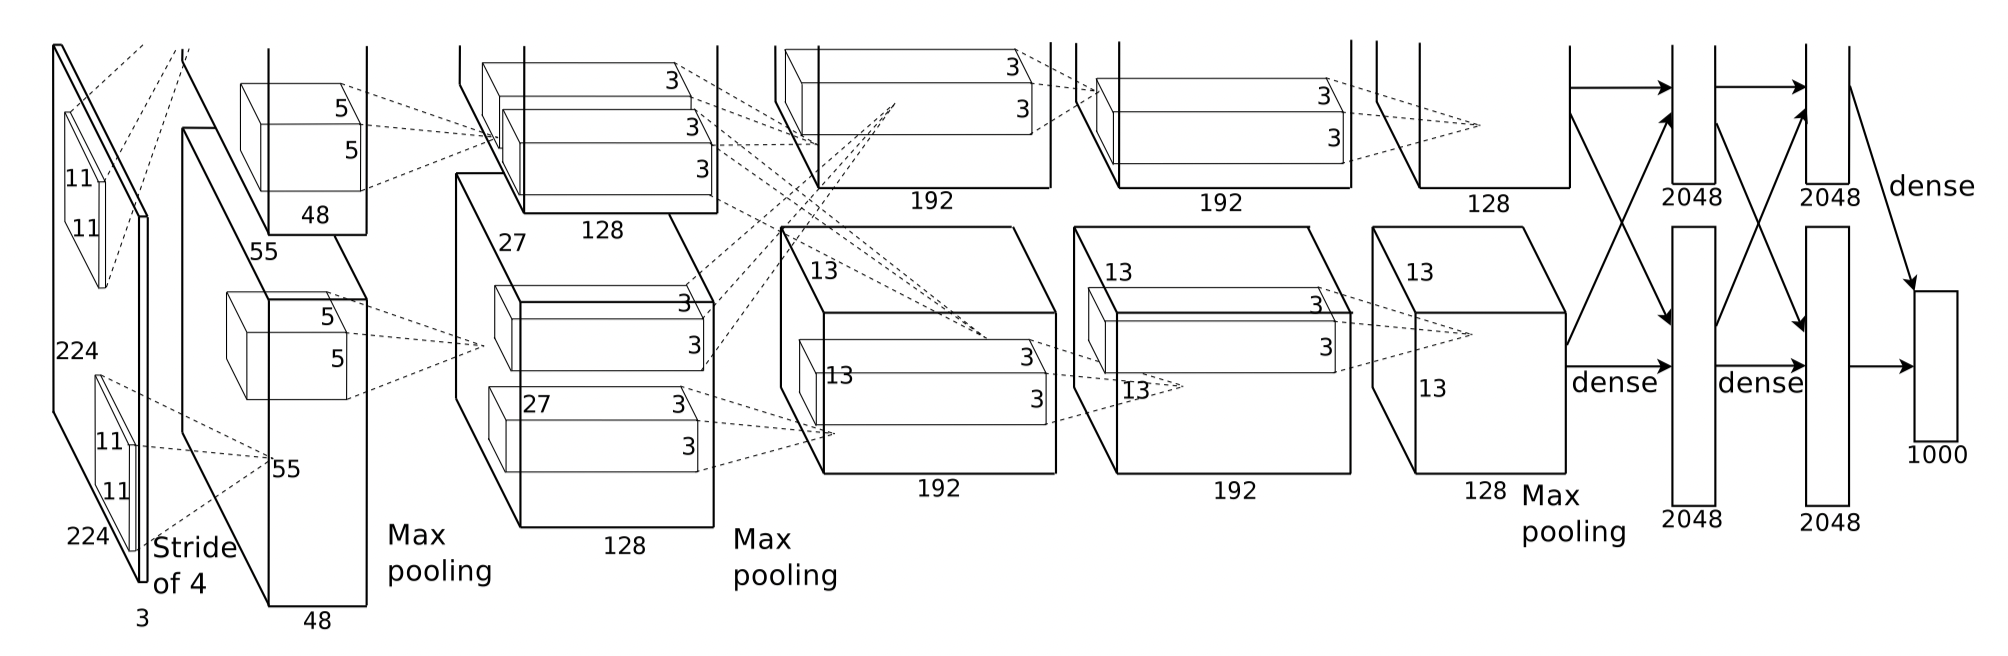
\includegraphics[width=6in]{figures/alex_net.png}
    \caption{AlexNet's Overall Architecture \cite{AlexNet_2017}} \label{fig:alex_net_architecture}
\end{figure}

In addition to being one of the largest networks and employing a parallelization strategy, AlexNet was among the first neural networks to employ ReLUs. The ReLUs activation function was employed instead of the more common $Tanh$ and $Sigmoid$ functions at the time because AlexNet was designed to reduce learning time. Using ReLUs, the model has a faster learning rate, which, according to the author, would vastly increase the performance of large models with a large data set. In addition, AlexNet implements local response normalization (LRN) to assist ReLUs in generalization. The non-trainable LRN layer is utilized following the first and second network layers. Following the first, second, and fifth layers, AlexNet employs a max-pooling layer with a size of 3 and a stride of two 2. The author notes that having an overlapping pooling layer — i.e., size 3 > stride 2 — decreases overfitting in general \cite{AlexNet_2017}.

AlexNet employs data augmentation and dropout techniques to address the issue of overfitting when training an extensive network with a large data set. For data augmentation, AlexNet randomly selects images into batches and resizes them to a resolution of $224 times 224$. It then generates a copy with horizontal reflection image transformation and a copy with modified intensity for the three RGB channels. The CPU generates these transformed images while the GPU trains on the previous batch, allowing the data augmentation process to be done without incurring any additional performance costs. In addition to data augmentation, AlexNet also uses the dropout technique. If the output of any hidden neurons is less than or equal to 0.5, the network sets its output to 0. This technique reduces the computation required because neurons with 0 need not be considered in the rest of the forward pass or updated during backpropagation. This method also permits neurons in the network to be independent of one another, as no neurons are guaranteed to persist with each training sample.

R-CNN model utilize the AlexNet architect implemented on the Caffe framework. R-CNN model pass each generated ROIs as seperated imaged to AlexNet for feature extraction. Since ROIs role is to find each object location in the image, thus AlexNet can assume each ROI only have exactly one object. AlexNet also require image input of fixed resolution $224 \times 224$, thus R-CNN transform to the required size by warping all pixels in a bounding box of $227 \times 227$.

\subsection{The Third Module: Classification With Pre-trained SVM}
After the second module, R-CNN is able to obtain multiple features for each ROI. Each ROI with extracted features then be given to each trained linear SVM classifier in each class for evaluation. Since each class has its own SVM classifier, thus the SVM only needs to distinguish between objects belonging to the class and objects that are not belonging to the class. Linear SVM classifier can be thought of as trying to draw a $N-1$ dimension separator in the $N$-dimension space where $N$ is the number of features of a specific class. The separator in SVM must be linear, and it tries to separate objects in the class and objects outside of the class. The best-fit separator has the highest margin between any point in the class and any point outside of the class. An example of 2-dimensional linear SVM is visualized by figure \ref{fig:2d_svm_viz} where the circle represents the object in this class, and the square is the object outside the class. Given that the class-specific SVM know what features the class possesses. The separation between objects in and out of the class can be done with little computation power, as we already have the extracted features. Each class SVM is then given the ROI a score representing the likelihood that the object in ROI belongs to this class. Therefore, for each ROI, the class with the highest SVM score is assigned to be the class for the object.

\begin{figure}[!ht]
    \centering
    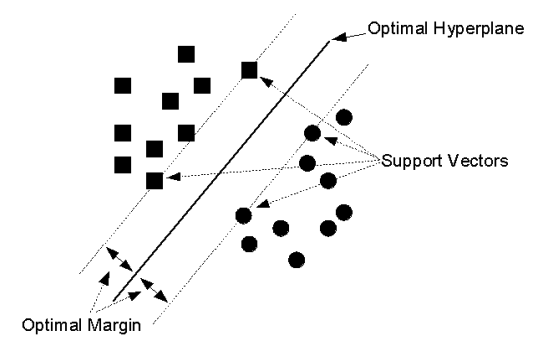
\includegraphics[height=2in]{figures/2d_svm.png}
    \caption{2D Linear SVM Visualization \cite{2d_svm_Tzotsos}} \label{fig:2d_svm_viz}
\end{figure}

\subsection{R-CNN Result and Drawback}
On the PASCAL VOC dataset 2012, by combining these three modules, R-CNN achieved 53.3\% in \textbf{mean Average Precision (mAP)}, a metric that measures the overall accuracy of the object detection network mentioned in Sec. {\color{red} Evaluation section number}. R-CNN also achieves the mAP of 31,4\% and ranks first on the ILSVRC2013 dataset in terms of accuracy \cite{Girshick_R_CNN_2013}. Despite achieving an incredible breakthrough in using Convolutional Networks and having a high object detection accuracy, R-CNN's performance is marred by a number of disadvantages. These issues include multi-stage training, high runtime and space complexity, reliance on non-learnable algorithms, and slowness \cite{fast_rcnn_og}. 

As described by the architecture of R-CNN, the network is divided into three modules and runs sequentially. The network attempts to feed the input of one module with the module's output coming before it. In other words, the first module must completely process the image before the second module is running. Therefore, the network's modules must wait on one another and be trained individually, thus creating the multi-stage training problem. Secondly, since the first module generates 2000 proposed ROIs before the second module can start running, the networks must cache these proposed ROIs on the disk. Similarly, the generated feature for each ROI must be stored on the disk before processing by SVM. The need to write and read multiple time for each ROI cause a high order of runtime and space complexity. The runtime and space complexity is even higher when we consider overlapping ROIs; the network recalculates features and classification for the overlapping portion of overlapping ROIs. Thirdly, the selective search algorithm used in the first module is a non-learnable algorithm. Therefore, the algorithm runtime and accuracy would not improve through training the network. Additionally, through the error analysis, the author notices the mass amount of localization inaccuracy. Thus, for each proposed region, after being scored by the SVMs, the region is piped to a class-specific bounding-box regressor to generate a new bounding box. Finding the bounding box within the region of interest allows the model to improve localization accuracy but exacerbates the model runtime performance as it generates the bounding box at least twice for each object in the image. Lastly, with a processing speed of 47s per image, the R-CNN model is slow and thus has limited real-world application.